\documentclass[11pt]{article}
\usepackage{amsmath}
\usepackage{amssymb}
\usepackage{graphicx}
\usepackage{tabularx}
\usepackage{fancyhdr}
\usepackage{lastpage}

% Page layout
\usepackage[top=1in, bottom=1in, left=1in, right=1in]{geometry}

% Header and footer
\pagestyle{fancy}
\fancyhf{}
\rfoot{Page \thepage}
\renewcommand{\headrulewidth}{0pt}

% Modified Question command with left-aligned number
\newcommand{\questiona}[2]{
    \noindent\textbf{Q#2.} #1 \hfill \textbf{[1 Mark]}
}

\newcommand{\questionb}[2]{
    \noindent\textbf{Q#2.} #1 \hfill \textbf{[2 Marks]}
}

\begin{document}

% Title section with horizontal line
\begin{center}
    \Large\textbf{GATE 2017 - Ecology and Evolution (EY)} \\
    \large\textbf{General Aptitude and Technical Questions} \\
    \rule{\textwidth}{0.5pt} % Horizontal line below heading
\end{center}

\vspace{0.5cm}

% General Aptitude Section
\section*{General Aptitude}

\questiona{She has a sharp tongue and it can occasionally turn \_\_\_\_\_}{56}
\begin{enumerate}
    \item[(A)] hurtful  
    \item[(B)] left  
    \item[(C)] methodical  
    \item[(D)] vital  
\end{enumerate}
\vspace{0.5cm}

\questiona{I \_\_\_\_\_ made arrangements had I \_\_\_\_\_ informed earlier.}{57}
\begin{enumerate}
    \item[(A)] could have, been  
    \item[(B)] would have, being  
    \item[(C)] had, have  
    \item[(D)] had been, been  
\end{enumerate}
\vspace{0.5cm}

\questiona{In the summer, water consumption is known to decrease overall by 25\%. A Water Board official states that in the summer household consumption decreases by 20\%, while other consumption increases by 70\%. Which of the following statements is correct?}{58}
\begin{enumerate}
    \item[(A)] The ratio of household to other consumption is 8/17  
    \item[(B)] The ratio of household to other consumption is 1/17  
    \item[(C)] The ratio of household to other consumption is 17/8  
    \item[(D)] There are errors in the official's statement.  
\end{enumerate}
\vspace{0.5cm}

\questiona{40\% of deaths on city roads may be attributed to drunken driving. The number of degrees needed to represent this as a slice of a pie chart is}{59}
\begin{enumerate}
    \item[(A)] 120  
    \item[(B)] 144  
    \item[(C)] 160  
    \item[(D)] 212  
\end{enumerate}
\vspace{0.5cm}

\questiona{Some tables are shelves. Some shelves are chairs. All chairs are benches. Which of the following conclusions can be deduced from the preceding sentences? \newline
i. At least one bench is a table \newline
ii. At least one shelf is a bench \newline
iii. At least one chair is a table \newline
iv. All benches are chairs}{60}
\begin{enumerate}
    \item[(A)] Only i  
    \item[(B)] Only ii  
    \item[(C)] Only ii and iii  
    \item[(D)] Only iv  
\end{enumerate}
\vspace{0.5cm}

\questionb{"If you are looking for a history of India, or for an account of the rise and fall of the British Raj, or for the reason of the cleaving of the subcontinent into two mutually antagonistic parts and the effects this mutilation will have in the respective sections, and ultimately on Asia, you will not find it in these pages; for though I have spent a lifetime in the country, I lived too near the seat of events, and was too intimately associated with the actors, to get the perspective needed for the impartial recording of these matters". \newline
Here, the word 'antagonistic' is closest in meaning to}{61}
\begin{enumerate}
    \item[(A)] impartial  
    \item[(B)] argumentative  
    \item[(C)] separated  
    \item[(D)] hostile  
\end{enumerate}
\vspace{0.5cm}

\questionb{S, T, U, V, W, X, Y, and Z are seated around a circular table. T's neighbours are Y and V. Z is seated third to the left of T and second to the right of S. U's neighbours are S and Y; and T and W are not seated opposite each other. Who is third to the left of V?}{62}
\begin{enumerate}
    \item[(A)] X  
    \item[(B)] W  
    \item[(C)] U  
    \item[(D)] T  
\end{enumerate}
\vspace{0.5cm}

\questionb{Trucks (10 m long) and cars (5 m long) go on a single lane bridge. There must be a gap of at least 20 m after each truck and a gap of at least 15 m after each car. Trucks and cars travel at a speed of 36 km/h. If cars and trucks go alternately, what is the maximum number of vehicles that can use the bridge in one hour?}{63}
\begin{enumerate}
    \item[(A)] 1440  
    \item[(B)] 1200  
    \item[(C)] 720  
    \item[(D)] 600  
\end{enumerate}
\vspace{0.5cm}

\questionb{There are 3 Indians and 3 Chinese in a group of 6 people. How many subgroups of this group can we choose so that every subgroup has at least one Indian?}{64}
\begin{enumerate}
    \item[(A)] 56  
    \item[(B)] 52  
    \item[(C)] 48  
    \item[(D)] 44  
\end{enumerate}
\vspace{0.5cm}

\questionb{A contour line joins locations having the same height above the mean sea level. The following is a contour plot of a geographical region. Contour lines are shown at 25 m intervals in this plot.}{65}
\begin{center}
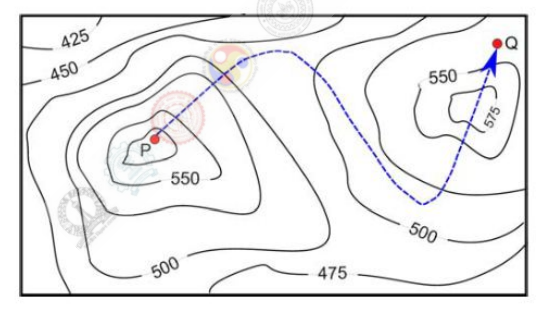
\includegraphics[width=0.5\textwidth]{figures/10.png}
\end{center}
The path from P to Q is best described by
\begin{enumerate}
    \item[(A)] Up-Down-Up-Down  
    \item[(B)] Down-Up-Down-Up  
    \item[(C)] Down-Up-Down  
    \item[(D)] Up-Down-Up  
\end{enumerate}
\vspace{0.5cm}

% Technical Section
\section*{Technical Section}

\questiona{The larvae of the monarch butterfly feed exclusively on milkweed plants. These larvae are relatively less susceptible to predation because they are:}{1}
\begin{enumerate}
    \item[(A)] Chemically protected  
    \item[(B)] Highly aggressive  
    \item[(C)] Protected by spines  
    \item[(D)] Visually cryptic  
\end{enumerate}
\vspace{0.5cm}

\questiona{Which one of the following evolutionary processes best describes Red Queen dynamics?}{2}
\begin{enumerate}
    \item[(A)] Co-evolution  
    \item[(B)] Convergent evolution  
    \item[(C)] Divergent evolution  
    \item[(D)] Parallel evolution  
\end{enumerate}
\vspace{0.5cm}

\questiona{Social behaviours can evolve to increase or decrease the fitness of the recipient of the behaviour. A behaviour is considered to be spiteful, when the fitness impact on the actor is \_\_\_\_\_, while the fitness impact on the recipient is \_\_\_\_\_.}{3}
\begin{enumerate}
    \item[(A)] negative; negative  
    \item[(B)] negative; positive  
    \item[(C)] positive; negative  
    \item[(D)] positive; positive  
\end{enumerate}
\vspace{0.5cm}

\questiona{Which of the following set of animals belongs to the group Afrotheria?}{4}
\begin{enumerate}
    \item[(A)] Elephant, dugong, elephant shrew, kangaroo rat  
    \item[(B)] Elephant, hyrax, elephant shrew, dugong  
    \item[(C)] Elephant, pika, hyrax, aardvark  
    \item[(D)] Elephant shrew, dugong, aardvark, pika  
\end{enumerate}
\vspace{0.5cm}

\questiona{What genetic markers are required to determine paternity in birds?}{5}
\begin{enumerate}
    \item[(A)] Microsatellites  
    \item[(B)] Mitochondrial DNA  
    \item[(C)] X chromosome markers  
    \item[(D)] Z chromosome markers  
\end{enumerate}
\vspace{0.5cm}

\questiona{Species 1 and 2 are sympatric, but species 2 has a wider physiological tolerance than species 1. The two species simultaneously invade a new environment that has an average temperature of 22 degrees C. What are the expected outcomes for species 1 and 2?}{6}
\begin{center}
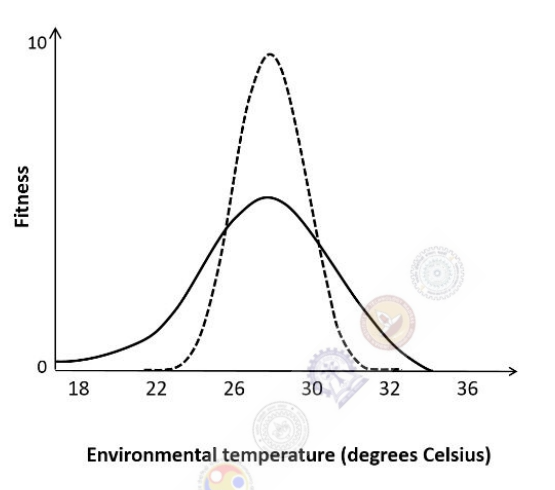
\includegraphics[width=0.5\textwidth]{figures/6.png}
\end{center}
\begin{enumerate}
    \item[(A)] Both species will survive in the long term  
    \item[(B)] Neither species will survive in the long term  
    \item[(C)] Species 1 will outcompete species 2  
    \item[(D)] Species 2 will outcompete species 1  
\end{enumerate}
\vspace{0.5cm}

\questiona{Plants have evolved many morphological adaptations to extreme environmental conditions. Which of the following is NOT an adaptation to desert life?}{7}
\begin{enumerate}
    \item[(A)] Dense coat of hairs or spines  
    \item[(B)] High density of stomata  
    \item[(C)] Photosynthetic stem  
    \item[(D)] Succulent or thick leaves  
\end{enumerate}
\vspace{0.5cm}

\questiona{When large mammals walk in the forest and trample small plants, those plants die. This interspecies relationship is a form of:}{8}
\begin{enumerate}
    \item[(A)] Amensalism  
    \item[(B)] Commensalism  
    \item[(C)] Mutualism  
    \item[(D)] Parasitism  
\end{enumerate}
\vspace{0.5cm}

\questiona{The population of a widely distributed species gets divided into two subpopulations due to the appearance of a mountain barrier. Eventually these subpopulations evolve into two separate species. This is a case of:}{9}
\begin{enumerate}
    \item[(A)] Allopatric speciation  
    \item[(B)] Parapatric speciation  
    \item[(C)] Peripatric speciation  
    \item[(D)] Sympatric speciation  
\end{enumerate}
\vspace{0.5cm}

\questiona{In a population, the frequency of genotypes at a locus are $A_1A_1 = 0.16$, $A_1A_2 = 0.48$, $A_2A_2 = 0.36$. The probability of fixation of the $A_1$ allele by genetic drift is \_\_\_\_\_.}{10}
\vspace{0.5cm}

\questiona{The percent sequence divergence in the mitochondrial \textit{Cytochrome b} gene between two species was found to be 5\%. Much of this divergence in the coding region would be contributed by changes at the:}{11}
\begin{enumerate}
    \item[(A)] First position of the codon  
    \item[(B)] Second position of the codon  
    \item[(C)] Third position of the codon  
    \item[(D)] Intron  
\end{enumerate}
\vspace{0.5cm}

\questiona{In haplo-diploid insects, males are haploid and females are diploid. A female, who is heterozygous for a recessive red-eye colour mutation, mates with a wild-type black-eyed male. What would be the percentage of eye colour phenotypes among their daughters?}{12}
\begin{enumerate}
    \item[(A)] 100\% red-eye  
    \item[(B)] 100\% black-eye  
    \item[(C)] 50\% red-eye  
    \item[(D)] 66.7\% black-eye  
\end{enumerate}
\vspace{0.5cm}

\questiona{What is the relationship between effective population size (Ne) and total population size (N) of any naturally occurring eukaryotic population?}{13}
\begin{enumerate}
    \item[(A)] Ne is greater than N  
    \item[(B)] Ne is less than N  
    \item[(C)] Ne is always equal to N  
    \item[(D)] Ne is unrelated to N  
\end{enumerate}
\vspace{0.5cm}

\questiona{The figure below represents the phylogenetic relationships of taxa P-S. Assuming that the branch lengths are proportional to divergence time, which among the following species pairs would be expected to show the most post-zygotic isolation?}{14}
\begin{center}
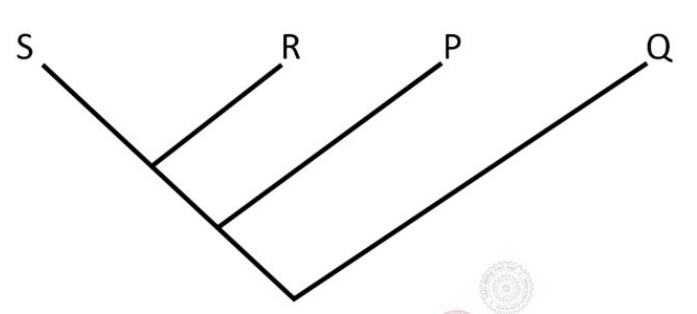
\includegraphics[width=0.5\textwidth]{figures/14.png}
\end{center}
\begin{enumerate}
    \item[(A)] P \& S  
    \item[(B)] Q \& R  
    \item[(C)] R \& P  
    \item[(D)] S \& R  
\end{enumerate}
\vspace{0.5cm}

\questiona{Members of which of the following animal phyla are exclusively marine?}{15}
\begin{enumerate}
    \item[(A)] Cnidaria  
    \item[(B)] Echinodermata  
    \item[(C)] Mollusca  
    \item[(D)] Porifera  
\end{enumerate}
\vspace{0.5cm}

\questiona{Some amphibians, such as axolotl larvae, rarely metamorphose into an adult form in spite of being sexually mature. This phenomenon of retention of larval characters in the adult form is known as:}{16}
\begin{enumerate}
    \item[(A)] Neoteny  
    \item[(B)] Ontogeny  
    \item[(C)] Pedogenesis  
    \item[(D)] Polyphenism  
\end{enumerate}
\vspace{0.5cm}

\questiona{Plants are classified into the following major categories: division, class, order and family. These four categories generally have specific suffixes. Which among the following describes the correct order of specific suffixes for the categories of division, class, order and family, respectively?}{17}
\begin{enumerate}
    \item[(A)] -ales, -opsida, -phyta, -aceae  
    \item[(B)] -opsida, -phyta, -aceae, -ales  
    \item[(C)] -phyta, -ales, -opsida, -aceae  
    \item[(D)] -phyta, -opsida, -ales, -aceae  
\end{enumerate}
\vspace{0.5cm}

\questiona{The Indian cricket team captain has lost the coin toss for nine consecutive games. Assuming that an unbiased coin is being used throughout the tournament, the chance that the Indian captain will win the toss on the $10^{th}$ game is \_\_\_\_\_.}{18}
\vspace{0.5cm}

\questiona{Consider the function $y = e^x$. The slope of this function at $x = 10$ is}{19}
\begin{enumerate}
    \item[(A)] 0  
    \item[(B)] 10  
    \item[(C)] $e^{10}$  
    \item[(D)] $10 e^{10}$  
\end{enumerate}
\vspace{0.5cm}

\questiona{Which of the following best demonstrates the phenomenon of a sign stimulus as defined in classical ethology? A male stickleback fish performing an aggressive display when presented with:}{20}
\begin{enumerate}
    \item[(A)] A diamond-shaped model with the lower half painted red  
    \item[(B)] A life-like model of a male stickleback fish with a red belly  
    \item[(C)] A mirror  
    \item[(D)] A video-recording of another male stickleback fish with a red belly  
\end{enumerate}
\vspace{0.5cm}

\questiona{Eating puffer fish can sometimes be fatal for human beings. This is because puffer fish carry a potent toxin known as:}{21}
\begin{enumerate}
    \item[(A)] Botulinum toxin  
    \item[(B)] Bungarotoxin  
    \item[(C)] Conotoxin  
    \item[(D)] Tetrodotoxin  
\end{enumerate}
\vspace{0.5cm}

\questiona{The 'Selfish Herd' hypothesis for group behavior predicts:}{22}
\begin{enumerate}
    \item[(A)] Competition among individuals for central positions in groups  
    \item[(B)] Competition among individuals for peripheral positions in groups  
    \item[(C)] Competition for food among individuals in groups  
    \item[(D)] Co-operative defence against predators  
\end{enumerate}
\vspace{0.5cm}

\questiona{Birds that inhabit forests typically produce calls in the form of low-pitched whistles. The most likely reason is that low-pitched whistles:}{23}
\begin{enumerate}
    \item[(A)] Are easy to localize  
    \item[(B)] Experience high levels of scattering  
    \item[(C)] Transmit over greater distances  
    \item[(D)] Travel faster than high-pitched whistles  
\end{enumerate}
\vspace{0.5cm}

\questiona{At mid-latitudes, which of the following biomes is associated with hot dry summers and cool rainy winters?}{24}
\begin{enumerate}
    \item[(A)] Boreal Forests  
    \item[(B)] Chapparal Forests  
    \item[(C)] Temperate Broadleaf Deciduous Forests  
    \item[(D)] Temperate Grasslands  
\end{enumerate}
\vspace{0.5cm}

\questiona{\textit{Rafflesia arnoldii} produces one of the largest flowers on earth and is typically pollinated by:}{25}
\begin{enumerate}
    \item[(A)] Bats  
    \item[(B)] Bees  
    \item[(C)] Birds  
    \item[(D)] Flies  
\end{enumerate}
\vspace{0.5cm}

\questionb{Lantana camara is an invasive weed introduced into India from South America. If you characterize the genetic variation of this species in both its native and introduced populations, the South American population is expected to have:}{26}
\begin{enumerate}
    \item[(A)] higher number of alleles per locus than the Indian population  
    \item[(B)] higher homozygosity than the Indian population  
    \item[(C)] lower number of alleles per locus than the Indian population  
    \item[(D)] lower genetic diversity than the Indian population  
\end{enumerate}
\vspace{0.5cm}

\questionb{Which of the following combination of properties of neuronal circuits mediating escape behaviour in animals would make them most effective at evading predators?}{27}
\begin{enumerate}
    \item[(A)] Large-diameter axons and chemical synapses  
    \item[(B)] Large-diameter axons and electrical synapses  
    \item[(C)] Small-diameter axons and chemical synapses  
    \item[(D)] Small-diameter axons and electrical synapses  
\end{enumerate}
\vspace{0.5cm}

\questionb{An experimentalist rejects a null hypothesis because she finds a $p$-value to be 0.01. This implies that:}{28}
\begin{enumerate}
    \item[(A)] There is a 1\% chance that the alternative hypothesis explains the data  
    \item[(B)] There is a 1\% chance that the null hypothesis explains the data  
    \item[(C)] There is a 99\% chance that the alternative hypothesis explains the data  
    \item[(D)] There is a 99\% chance that the null hypothesis explains the data  
\end{enumerate}
\vspace{0.5cm}

\questionb{A student counts every individual blackbuck in two grasslands. He finds 2100 and 2300 blackbuck in the two areas. Which statistical test is required to establish that these two population sizes are different?}{29}
\begin{enumerate}
    \item[(A)] Chi-square test  
    \item[(B)] F-test  
    \item[(C)] No test is required  
    \item[(D)] Student's t-test  
\end{enumerate}
\vspace{0.5cm}

\questionb{The plot below shows the fitness of two traits as a function of relative frequency of trait-1 in the population. The solid line represents the fitness of trait-1 and the dotted line represents the fitness of trait-2. Which of the following is most likely to be TRUE?}{30}
\begin{center}
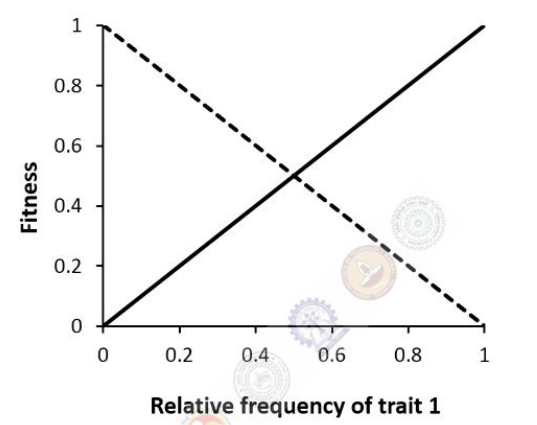
\includegraphics[width=0.5\textwidth]{figures/30.png}
\end{center}
\begin{enumerate}
    \item[(A)] Either Trait-1 or Trait-2 will take over the population  
    \item[(B)] Only Trait-1 will take over the population  
    \item[(C)] Trait-1 and Trait-2 will always reach a coexistence equilibrium  
    \item[(D)] Trait-1 and Trait-2 will oscillate over time  
\end{enumerate}
\vspace{0.5cm}

\questionb{The following figure shows the phylogeny of insect species 1-5. Each of these 5 insect species harbors a specific bacterial endosymbiont. S, R, Q, T and P are the endosymbiont bacteria associated with insect species 1, 2, 3, 4 and 5, respectively. Which one of the following symbiont phylogenetic trees suggests host shift by these endosymbionts?}{31}
\begin{center}
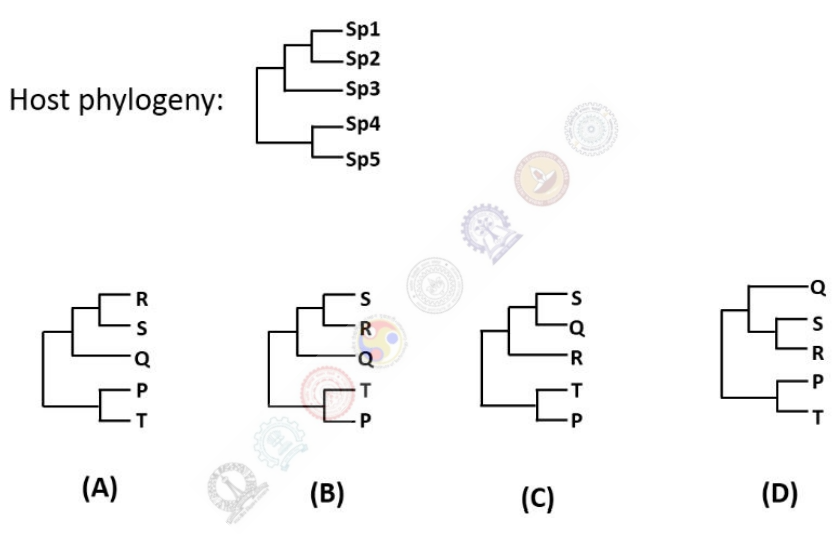
\includegraphics[width=0.9\textwidth]{figures/31.png}
\end{center}
\vspace{0.5cm}

\questionb{P to T are islands of different sizes at different distances from the mainland, where the distance $x < y < z$. The area of island $P > Q > R = S = T$. Assuming that there is migration only from the mainland to islands and not between islands, which of the following is NOT true about species richness on these islands?}{32}
\begin{center}
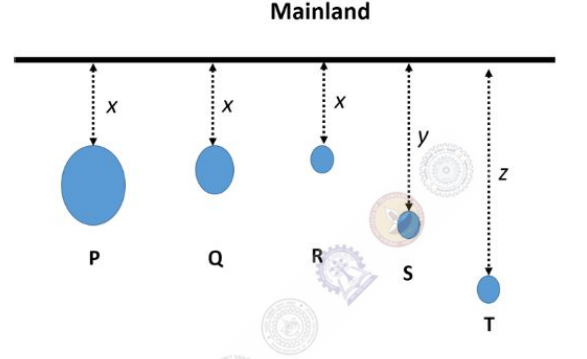
\includegraphics[width=0.5\textwidth]{figures/32.png}
\end{center}
\begin{enumerate}
    \item[(A)] $P > Q > R$  
    \item[(B)] $R > S > T$  
    \item[(C)] $Q > T > S$  
    \item[(D)] $S < Q < P$  
\end{enumerate}
\vspace{0.5cm}

\questionb{The frequency of an allele at a locus on the non-recombining region of the Y chromosome in humans is 0.3. If the population size is N and the sex ratio is 1:1, what is the number of copies of the alleles in the population?}{33}
\begin{enumerate}
    \item[(A)] 0.3 N/4  
    \item[(B)] 0.3 N/2  
    \item[(C)] 0.3 N  
    \item[(D)] 0.6 N  
\end{enumerate}
\vspace{0.5cm}

\questionb{The species compositions of three areas, P, Q and R are shown below: \newline
P: Cobra, Gecko, Crow, Viper \newline
Q: Viper, Tiger, Salamander, Fish \newline
R: Salamander, Viper, Frog, Chameleon \newline
Based on the relationship between species, one can determine the phylogenetic diversity of each region. Which of the following captures the order of phylogenetic diversity of these regions?}{34}
\begin{enumerate}
    \item[(A)] $Q > P = R$  
    \item[(B)] $Q = R > P$  
    \item[(C)] $Q > R > P$  
    \item[(D)] $R > Q > P$  
\end{enumerate}
\vspace{0.5cm}

\questionb{Recent paleogenomic studies indicate that some groups of living humans have Neanderthal genes in their genomes. What is the best explanation for this phenomenon?}{35}
\begin{enumerate}
    \item[(A)] Modern humans descended directly from Neanderthals  
    \item[(B)] Neanderthals are still living among us  
    \item[(C)] Some genes in modern humans have reverted to Neanderthal-like sequences  
    \item[(D)] Some ancestors of living humans hybridized with the Neanderthals  
\end{enumerate}
\vspace{0.5cm}

\questionb{A population grows as per the equation $\frac{dn}{dt} = r \, n \, (1 - n/1000)$ where $n$ is the population density, $r$ is the intrinsic growth rate and 1000 is the carrying capacity. The growth rate of the population is maximum at a population density of \_\_\_\_\_.}{36}
\vspace{0.5cm}

\questionb{An ecology exam paper has a large number of multiple choice questions with five options each, of which only one is correct. An unprepared student picks one of the five given options randomly, and attempts all questions. A correct answer yields one mark whereas a wrong answer yields negative $x$ mark(s). To ensure that an unprepared student most likely gets zero marks, the value of $x$ must be \_\_\_\_\_ (write only the magnitude, not the sign).}{37}
\vspace{0.5cm}

\questionb{Increasing atmospheric CO$_2$ concentration is likely to benefit C3 plants more than C4 plants because:}{38}
\begin{enumerate}
    \item[(A)] C4 photosynthesis is inhibited by increasing CO$_2$  
    \item[(B)] Carboxylation increases relative to oxygenation in C3 plants  
    \item[(C)] Oxygenation is suppressed in C4 plants  
    \item[(D)] Transpiration increases with increasing CO$_2$ in C4 plants  
\end{enumerate}
\vspace{0.5cm}

\questionb{In metacommunities composed of species A and B, the rates of colonization of habitat patches by A and B are C$_A$ and C$_B$. The rates of extinction for species A and B in the absence of competition, are E$_A$ and E$_B$. Species A is the superior competitor within any given patch. Which one of the following conditions is necessary to allow the continued persistence of species B?}{39}
\begin{enumerate}
    \item[(A)] E$_A$ $>$ E$_B$  
    \item[(B)] C$_B$/E$_B$ $>$ C$_A$/E$_A$  
    \item[(C)] C$_B$/E$_B$ $<$ C$_A$/E$_A$  
    \item[(D)] C$_B$ $>$ C$_A$  
\end{enumerate}
\vspace{0.5cm}

\questionb{Batesian and Müllerian mimicry are effective anti-predatory defences because predators show:}{40}
\begin{enumerate}
    \item[(A)] Habituation  
    \item[(B)] Imprinting  
    \item[(C)] Learning by negative reinforcement  
    \item[(D)] Learning by positive reinforcement  
\end{enumerate}
\vspace{0.5cm}

\questionb{A species possesses ten types of olfactory receptors (encoded by ten unique gene sequences) but is able to perceptually distinguish a hundred different odorants. This is possible because each olfactory receptor type:}{41}
\begin{enumerate}
    \item[(A)] binds to a subset of the 100 odorant molecules with unequal affinities  
    \item[(B)] binds to all 100 types of odorant molecules with equal affinity  
    \item[(C)] changes its specificity in relation to the odorant molecule  
    \item[(D)] is specific and binds only one species of odorant molecule  
\end{enumerate}
\vspace{0.5cm}

\questionb{Among vertebrates, male-only parental care is more commonly found among fishes and amphibians than birds and mammals. The most likely reason for this is because fishes and amphibians are characterised by:}{42}
\begin{enumerate}
    \item[(A)] External fertilization  
    \item[(B)] Moist skin  
    \item[(C)] Poikilothermy  
    \item[(D)] Sexual dimorphism  
\end{enumerate}
\vspace{0.5cm}

\questionb{Guppies are fish that typically have blue, red and yellow spots on their bodies. In an experiment, one group of guppies was subjected to treatment X, where they were maintained and allowed to breed for several generations in ponds containing their natural predator species. A second group of fish was subjected to treatment Y, where they were maintained and allowed to breed for the same number of generations in ponds from which all predators were removed. After several generations, it was found that guppies subjected to treatment X had lost their blue spots, whereas those subjected to treatment Y showed an increase in the number of blue spots. Based on these observations, which one of the following statements can be rejected?}{43}
\begin{enumerate}
    \item[(A)] Blue spots on guppies are subject to natural selection  
    \item[(B)] Blue spots on guppies may be subject to sexual selection  
    \item[(C)] Blue spots are likely to make guppies more conspicuous to predators  
    \item[(D)] Blue spots are likely to make guppies less conspicuous to predators  
\end{enumerate}
\vspace{0.5cm}

\questionb{Which of the following is NOT a plausible explanation for the evolution of seed dispersal mechanisms in plants?}{44}
\begin{enumerate}
    \item[(A)] Long-distance dispersal benefits the dispersal agent  
    \item[(B)] Seed dispersal agents carry seeds to areas favourable for germination  
    \item[(C)] Seeds falling close to the parent plant have a higher risk of predation  
    \item[(D)] The area close to the parent plant is not optimal because of competition with kin  
\end{enumerate}
\vspace{0.5cm}

\questionb{Which of the following evolutionary changes was NOT associated with the colonization of land by plants?}{45}
\begin{enumerate}
    \item[(A)] Acquisition of dynein-mediated transport  
    \item[(B)] Acquisition of Jasmonic acid signaling  
    \item[(C)] Acquisition of vasculature  
    \item[(D)] Acquisition of seed desiccation tolerance  
\end{enumerate}
\vspace{0.5cm}

\questionb{For a given low population size, which of these plant species are more likely to experience Allee effects?}{46}
\begin{enumerate}
    \item[(A)] Asexual plants  
    \item[(B)] Bisexual plants  
    \item[(C)] Dioccious plants  
    \item[(D)] Monoccious plants  
\end{enumerate}
\vspace{0.5cm}

\questionb{Which of the following combinations of leaf traits is most likely to be observed in terrestrial plant communities that occur in low-nutrient environments with herbivory?}{47}
\begin{enumerate}
    \item[(A)] High levels of protein and high levels of chemical defences  
    \item[(B)] High levels of protein and low levels of chemical defences  
    \item[(C)] Low levels of protein and high levels of chemical defences  
    \item[(D)] Low levels of protein and low levels of chemical defences  
\end{enumerate}
\vspace{0.5cm}

\questionb{Which of the following sets of parameters form the basis of Holdridge's lifezone classification?}{48}
\begin{enumerate}
    \item[(A)] Altitude, Mean Annual Biotemperature, Annual Precipitation  
    \item[(B)] Annual Precipitation, Mean Annual Biotemperature, Length of dry season  
    \item[(C)] Potential Evapotranspiration, Annual Maximum Temperature, Annual Precipitation  
    \item[(D)] Potential Evapotranspiration Ratio, Mean Annual Biotemperature, Annual Precipitation  
\end{enumerate}
\vspace{0.5cm}

\questionb{The Annual Net Primary Productivity (ANPP) of ecosystems varies with the type of biome. Which of the following represents the correct order of ANPP values?}{49}
\begin{enumerate}
    \item[(A)] $Temperate Broadleaf Forest > Tropical Moist Forest > Boreal Forest > Savanna  $
    \item[(B)] $Tropical Moist Forest > Savanna > Temperate Broadleaf Forest > Boreal Forest$  
    \item[(C)] $Tropical Moist Forest > Temperate Broadleaf Forest > Boreal Forest > Savanna$  
    \item[(D)] $Tropical Moist Forest > Temperate Broadleaf Forest > Savanna > Boreal Forest$  
\end{enumerate}
\vspace{0.5cm}

\questionb{Which of these communities (R1, R2, R3, and R4), each with 80 species and represented by their Species Rank-Abundance curves, is likely to have the highest value of Shannon's index of species diversity?}{50}
\begin{center}
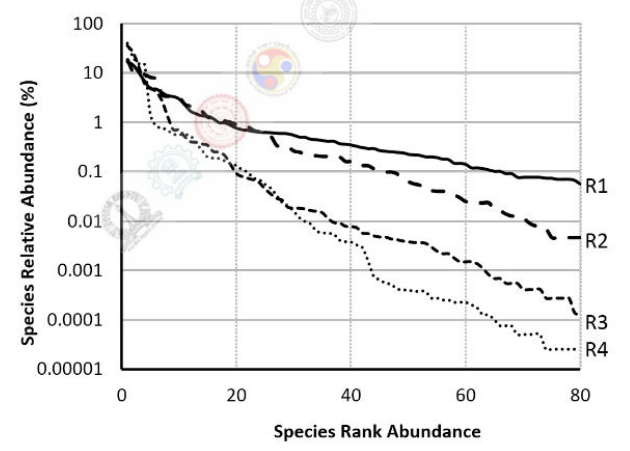
\includegraphics[width=0.5\textwidth]{figures/50.png}
\end{center}
\begin{enumerate}
    \item[(A)] R1  
    \item[(B)] R2  
    \item[(C)] R3  
    \item[(D)] R4  
\end{enumerate}
\vspace{0.5cm}

\questionb{In any experimental design, we prefer a large sample size because:}{51}
\begin{enumerate}
    \item[(A)] It reduces errors in the estimation of the mean effect  
    \item[(B)] It reduces the possibility of outliers  
    \item[(C)] It reduces type-I errors  
    \item[(D)] It reduces variability between different data points  
\end{enumerate}
\vspace{0.5cm}

\questionb{In haplo-diploid insects, males are haploid and females are diploid. For a haplo-diploid species, assume that each individual mates only once. The minimum coefficient of relatedness between two female cousins, whose maternal grandmother is the same, is \_\_\_\_\_ (enter answer to 4 decimal places).}{52}
\vspace{0.5cm}

\questionb{Match the scientists with the concepts or theories they are most famously associated with:}{53}
\begin{center}
\begin{tabular}{|l|l|}
\hline
P: & Gause \\ \hline
Q: & Hamilton \\ \hline
R: & Paine \\ \hline
S: & MacArthur \\ \hline
\end{tabular}
\begin{tabular}{|l|l|}
\hline
i: & Keystone species \\ \hline
ii: & Island biogeography \\ \hline
iii: & Kin selection \\ \hline
iv: & Competitive exclusion \\ \hline
\end{tabular}
\end{center}
\begin{enumerate}
    \item[(A)] $P - i$; $Q - iii$; $R - iv$; $S - ii$  
    \item[(B)] $P - iv$; $Q - iii$; $R - ii$; $S - i$  
    \item[(C)] $P - iv$; $Q - iii$; $R - i$; $S - ii$  
    \item[(D)] $P - iv$; $Q - i$; $R - ii$; $S - iii$  
\end{enumerate}
\vspace{0.5cm}

\questionb{Which of the following graphs best represents the function given by the following equation:}{54}
\begin{center}
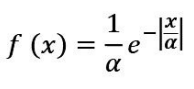
\includegraphics[width=0.2\textwidth]{figures/54a.png}
\end{center}
\begin{center}
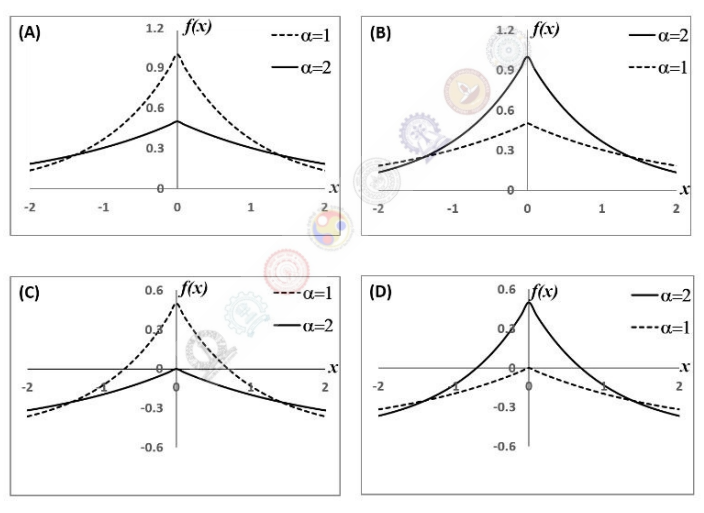
\includegraphics[width=0.9\textwidth]{figures/54.png}
\end{center}

\questionb{On the semi-arid plateaus of the Western Ghats, raptors, lizards, and grasshoppers dominate the community of animals. Raptors prey primarily on lizards, which prey primarily on grasshoppers. If raptor density declines significantly, which of the following is expected?}{55}
\begin{enumerate}
    \item[(A)] Both grasshopper and plant densities will increase  
    \item[(B)] Only grasshopper density will increase  
    \item[(C)] Plant density will increase  
    \item[(D)] Plant density will decrease  
\end{enumerate}
\vspace{0.5cm}

\vspace{0.5cm}
\begin{center}
\textbf{END OF THE QUESTION PAPER} \\
\rule{\textwidth}{0.5pt}
\end{center}

\end{document}
